\documentclass[titlepage]{article}\usepackage{babel}\usepackage{amsmath}\usepackage{amssymb}\usepackage{amsthm}\usepackage{multicol}\usepackage{graphicx}\usepackage[normalem]{ulem}\usepackage{tabto}\usepackage{hyperref}\usepackage{tikz}\usepackage{pgfplots}\pgfplotsset{compat=1.15}\usepackage{mathrsfs}\usetikzlibrary{arrows}\usetikzlibrary{shapes.geometric}\usepackage{wasysym}\usepackage{bbm}\usepackage{bbold}\usepackage{xcolor}\usepackage[T1]{fontenc}\usepackage{mathrsfs}\usepackage[utf8]{inputenc}\usepackage{listings}\pagestyle{plain}\pagenumbering{arabic}\renewcommand{\arraystretch}{1.3}\newcommand{\n}{\newline}\usepackage[left=20mm, right=15mm, top=25mm, bottom=7mm, paper=a4paper]{geometry}\renewcommand{\contentsname}{Inhaltsverzeichnis}\newcommand{\K}{\mathbb{K}}\newcommand{\C}{\mathbb{C}}\newcommand{\N}{\mathbb{N}}\newcommand{\Q}{\mathbb{Q}}\newcommand{\R}{\mathbb{R}}\newcommand{\1}{\mathbb{1}}\newcommand{\0}{\mathbb{0}}\newcommand{\Z}{\mathbb{Z}}\renewcommand{\)}{\right)}\renewcommand{\(}{\left(}

\begin{document}
	\begin{center}
		\begin{center}
			\LARGE\textsc{Diskrete Strukturen - Übung 11} \normalsize
		\end{center}
		\hrulefill\\
		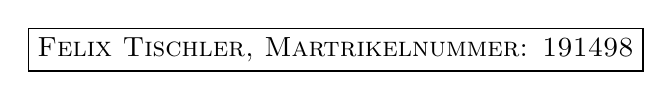
\begin{tikzpicture}
			\draw (0,0) node[draw, rectangle]{\textsc{Felix Tischler, Martrikelnummer: 191498}};
		\end{tikzpicture}
		\date{\today}
	\end{center}
	
	\part*{Relation}
	1.) Es sei $[M,\le]$ eine halbgeordnete Menge und $A\subseteq M$.\\\\
	\indent a)
	\begin{enumerate}
		\item []
		\begin{enumerate}
			\item[$\circ$)] $x\in M$ ist \textbf{untere Schranke} von A$\leftrightarrow_{df}\underset{a\in A}{\bigwedge}(a\ge x)$ \\
			\item[$\circ$)] $x\in M$ ist \textbf{Minimum} von A$\leftrightarrow_{df}$ es gilt: \\ 1.) "$x$ ist untere Schranke von $A$" und 2.) $x\in A$ \\
			\item[$\circ$)] $x\in M$ ist \textbf{Infimum} von A$\leftrightarrow_{df}$ es gilt: \\ 1.) "$x$ ist untere Schranke von A" und 2.) $\underset{y\in M}{\bigwedge}\(\underset{a\in A}{\bigwedge}(a\ge y)\rightarrow x\ge y\right)$ \\
			\item[$\circ$)] $x\in M$ ist \textbf{minimales Element} von A$\leftrightarrow_{df}$ es gilt: \\ 1.) $x\in A$ und 2.) es gibt kein Element $z\in A$ mit $z\neq x$ und $x\ge z$
		\end{enumerate}
	\end{enumerate}
	
	\indent b)
	\begin{enumerate}
		\item[]Beispiel 1: $[\R,\le]$ : Es sei $A=\R$. $A$ \textit{besitzt \underline{keine} \textbf{untere Schranken}, folglich kein \textbf{Minimum} und kein \textbf{Infimum}, aber auch keine \textbf{minimalen Elemente}.}
		\item[]Beispiel 2: $[\N,\le]$ : $A=\{0,1,2\}$. Untere Schranken sind $0,-1,-2,-3...$. Die $0$ \textit{ist \textbf{untere Schranke}, \textbf{minimales Element}, \textbf{Minimum} und \textbf{Infimum}.}\\
	\end{enumerate}
	
	\noindent
	2.) Wir wissen: Die Menge der natürlichen Zahlen $\N$ zusammen mit der üblichen kleiner-gleich-Relation $\le$ ist eine halbgeordnete Menge $[\N,\le]$
	\begin{table}[h]
		\begin{tabular}{l|c|c|c}
			Fall:&$m\le n$&$n\le m$&$m=n$\\\hline
			 $Sup_{\le}(\{m,n\})$&$n$&$m$&$max\{m,n\}$\\
			 $Inf_{\le}(\{m,n\})$&$m$&$n$&$min\{m,n\}$
		\end{tabular}
	\end{table}

	\noindent Fall 1 und 2 sind wohldefiniert, Fall 3 ebenfalls, da Maximum und Minimum immer existieren.
	\\\\
		
	\noindent
	3.) Wir wissen: Die Menge der natürlichen Zahlen $\N$ zusammen mit der üblichen Teilerrelation $\textbackslash$ ist eine halbgeordnete Menge $[\N,\textbackslash]$
	\begin{enumerate}
		\item[]$Sup_{\textbackslash}(\{m,n\})=kgV(m,n)$, da $m\mid kgV(m,n)$ und $n\mid kgV(m,n)$, denn "kleinste" im Namen bedeutet dass es sich um die kleinste obere Schranke handelt.
		\item[]$Inf_{\textbackslash}(\{m,n\})=ggT(m,n)$, da $ggT(m,n)\mid m$ und $ggT(m,n)\mid n$, denn "größte" im Namen bedeutet dass es sich um die größte untere Schranke handelt.
	\end{enumerate}
	\noindent Falls $m$ und $n$ teilerfremd sind, haben sie zumindest 1 als $ggT$ und das $kgV$ ist höchstens $m\cdot n$. Beides existiert immer.
	\\\\
	\noindent
	4.) Wir wissen: Die Menge der natürlichen Zahlen $\N$ zusammen mit der üblichen Teilmengenbeziehung $\subseteq$ ist eine halbgeordnete Menge $[\mathscr{P}(M),\subseteq]$
	\begin{enumerate}
		\item[]$Sup_{\subseteq}(X,Y)=X\cup Y$, wenn man ein Element wegnehmen würde, wäre die Relation nicht mehr gegeben, d.h. es handelt sich hierbei um die kleinste Schranke.
		\item[]$Inf_{\subseteq}(X,Y)=X\cap Y$, wenn man ein Element hinzugeben würde, wäre die Relation nicht mehr gegeben, d.h. es handelt sich hierbei um die größte Schranke.
	\end{enumerate}
	\noindent Schnitt und Vereinigung existieren immer.
	
\end{document}
